\documentclass[a4paper]{article}
\usepackage[letterpaper, margin=1in]{geometry} % page format
\usepackage{listings,graphicx,amsmath, amssymb, amsfonts, amsthm,tikz,hyperref,fullpage,setspace,enumerate,mathtools,arydshln} 

\title{Homework 3}
\author{Helen Ngo}
\date{\today}

\begin{document}
\lstset{language=Python}

\maketitle

\begin {description}

\item[Problem 1] Compare two algorithms on a classification task: the Pocket algorithm (designed for classification), and linear regression (not designed for classification). For linear regression, after learning the weights $\textbf{w}$; we use $h(\textbf{x}) = \textrm{sign}(\textbf{w}^T\textbf{x})$ to classify $\textbf{x}$. For the dataset, start by using the given code. Then create another dataset using the same methods as above, which we will use to estimate $E_{out}$. Try the following three approaches using multiple randomized experiments and explain which works best in terms of both $E_{out}$ and the amount of computation required. 

\begin{enumerate}[(a)]
\item The Pocket algorithm, starting from $\textbf{w} = 0$.
\item Linear regression (applied as a classification method).
\item The Pocket algorithm, starting from the solution given by linear regression.
\end{enumerate}

Also, try adding some $significant$ outliers to the $y = +1$ class (arbitrarily chosen) of the training dataset and explain how that affects your results.

\smallskip

\textbf{Solution:}
\begin{doublespace}
Several trials were conducted with samples sizes of $500$. In each of the trials, a dataset was created and all three of the approaches above were used. The datasets were created using the generate points functions and the Python code given:


\lstinputlisting[language=Python, firstline=15, lastline=45, frame=single]{pocket.py}

\newpage
Since Trials 1 and 4 best summarize the difference between random linearly separable and inseparable datasets, they will be further analyzed below, but the final hypothesis for every dataset and algorithm combination can be seen in the Github repository. In Trial 1, a linearly inseparable dataset was produced:
\begin{center}
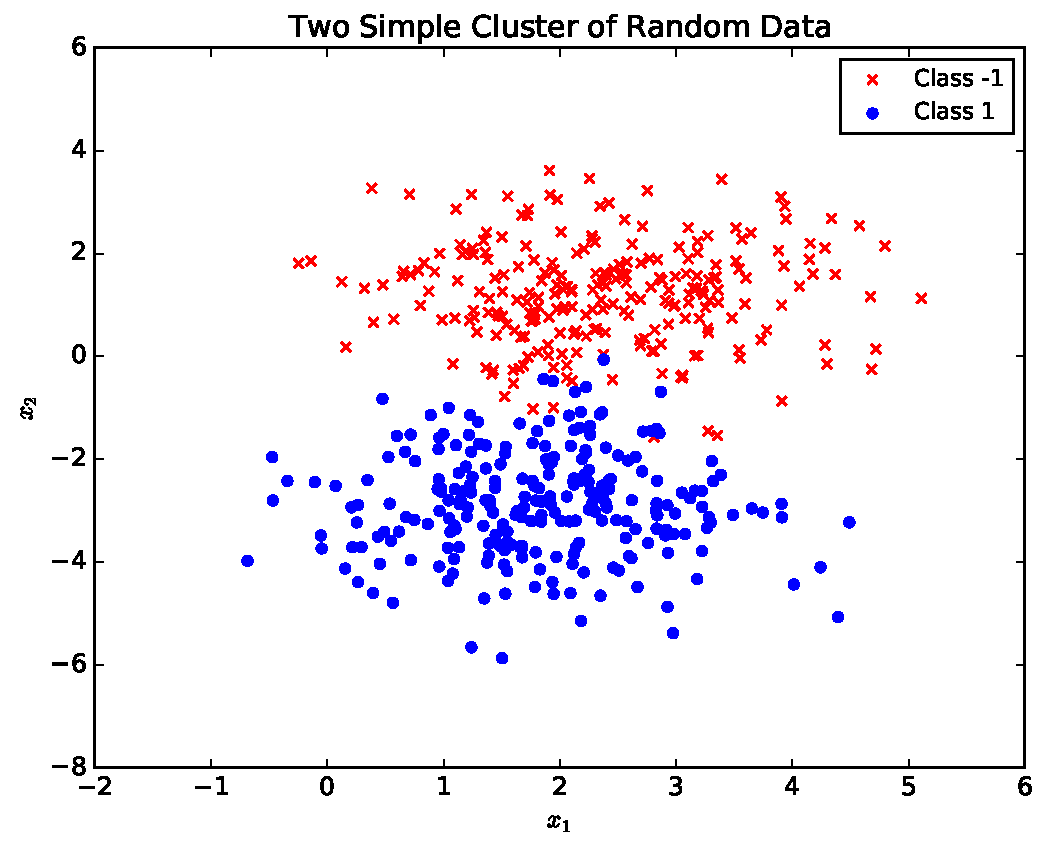
\includegraphics[scale=0.65]{Trial_1/hw3_plot.pdf}
\end{center}
For this dataset, it took
\begin{enumerate}[(a)]
\item the Pocket algorithm $723$ iterations and approximately $9$ seconds to converge,
\begin{center}
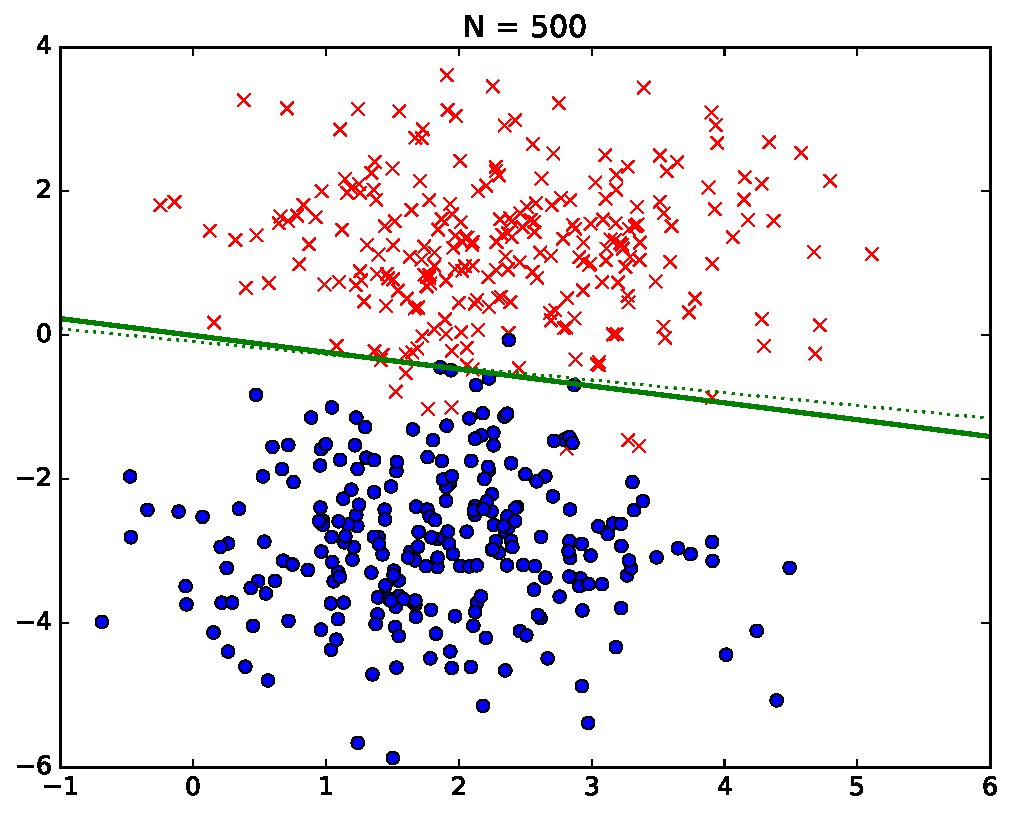
\includegraphics[scale=0.5]{Trial_1/pocket_learning.pdf}
\end{center}
\item the linear regression $3$ second to find a hypothesis, and 
\begin{center}
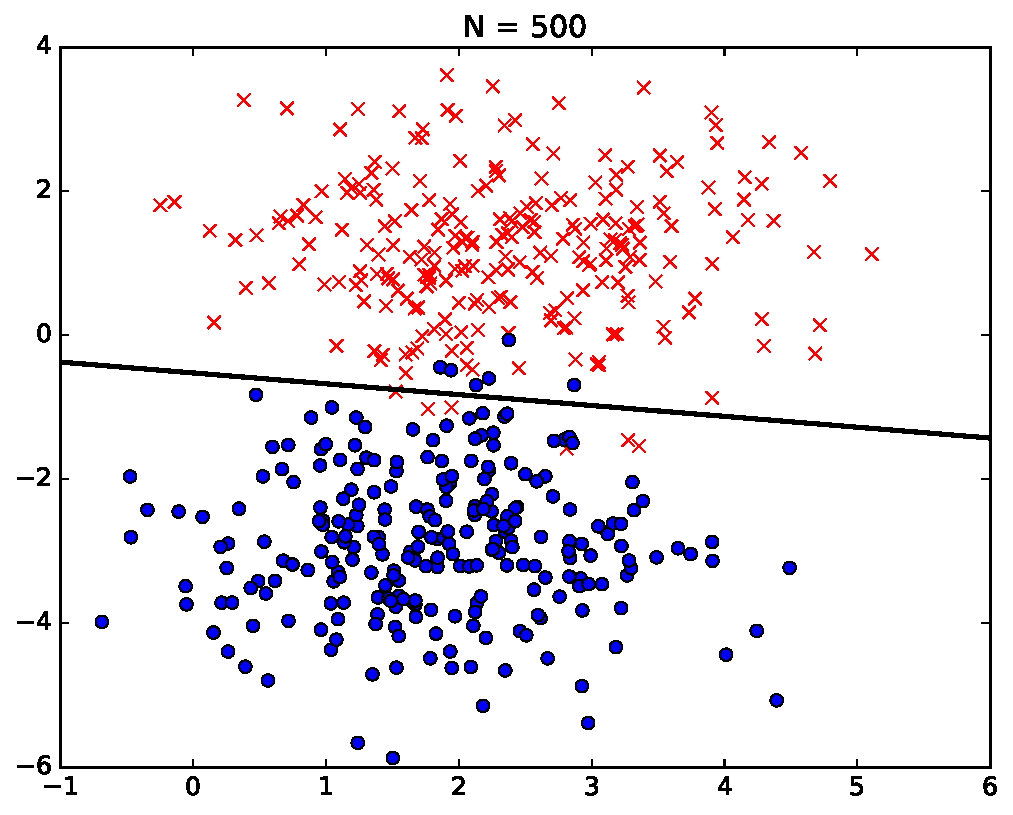
\includegraphics[scale=0.5]{Trial_1/linear_regression.pdf}
\end{center}
\item  the Pocket algorithm using the linear regression solution, $528$ iterations and $7$ seconds to converge.
\begin{center}
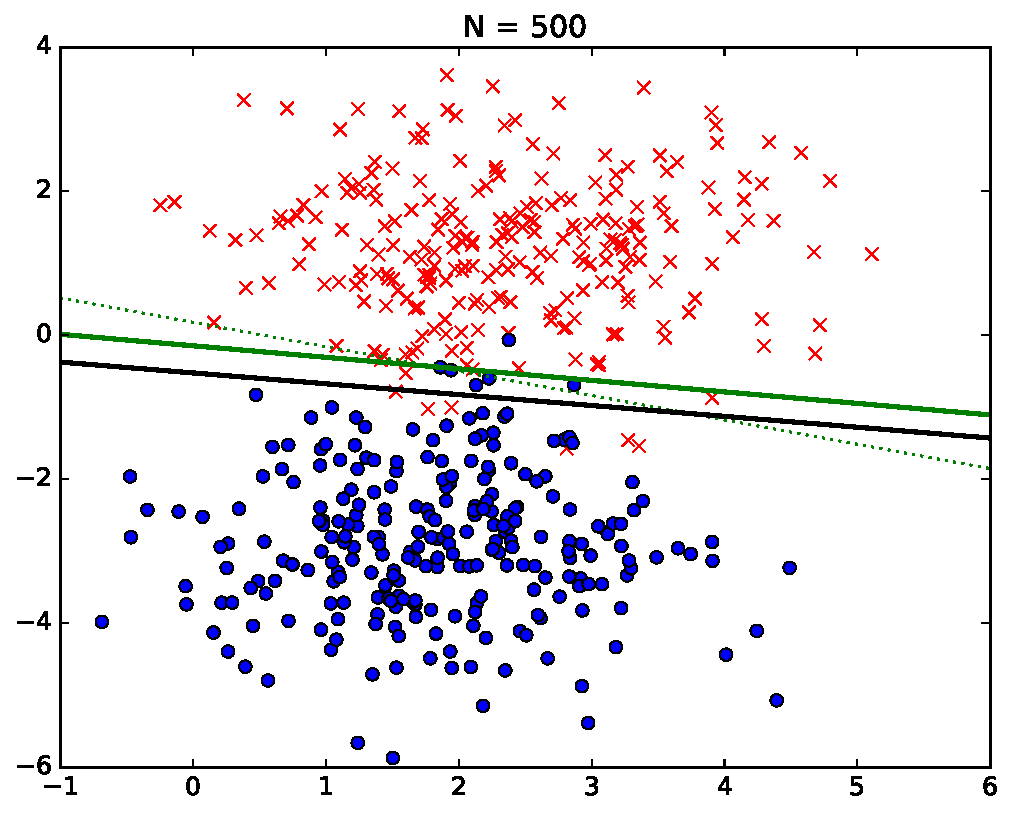
\includegraphics[scale=0.5]{Trial_1/pocket_with_lr.pdf}
\end{center}
\end{enumerate}

It should be noted that convergence is either no classification error, more than 500 iterations with the same optimal hypothesis, or more than ten thousand total iterations, which can be seen in the pla function.

\lstinputlisting[language=Python, firstline=121, lastline=148,frame=single]{pocket.py}

Taking into account how convergence is defined in the code, and what we know about the dataset, we can say that while there is no solution without misclassification, the Pocket algorithms produce hypotheses with lower $E_{out}$, but at a greater computational cost. For this specific example, the linear regression provides a similar $E_{out}$ result to Pocket algorithms but less than half the computation required. We can see from the plot associated with (c) the Pocket algorithm starting from the solution given by linear regression, that an improvement was made to $E_{out}$ to that of just the linear regression.

\newpage
In Trial 4, a linearly separable dataset was produced: 
\begin{center}
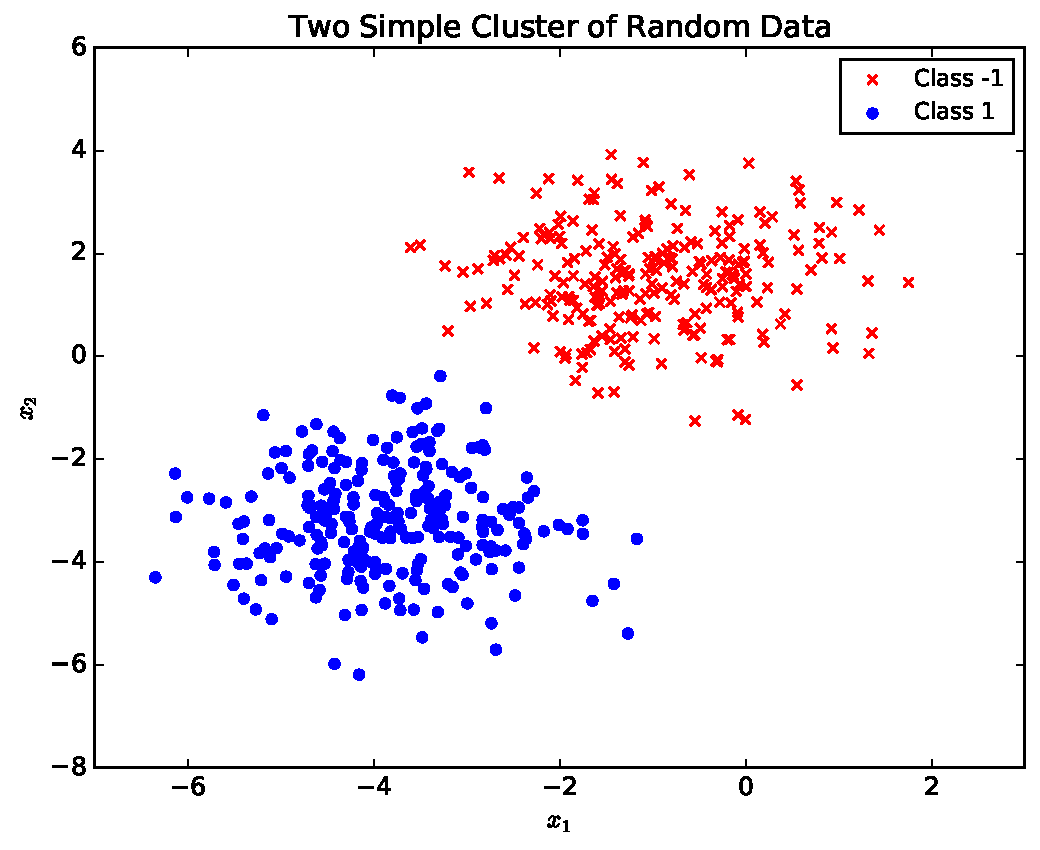
\includegraphics[scale=0.65]{Trial_4/hw3_plot.pdf}
\end{center}
For this dataset, it took
\begin{enumerate}[(a)]
\item the Pocket algorithm $21$ iterations and approximately $2$ seconds to converge,
\begin{center}
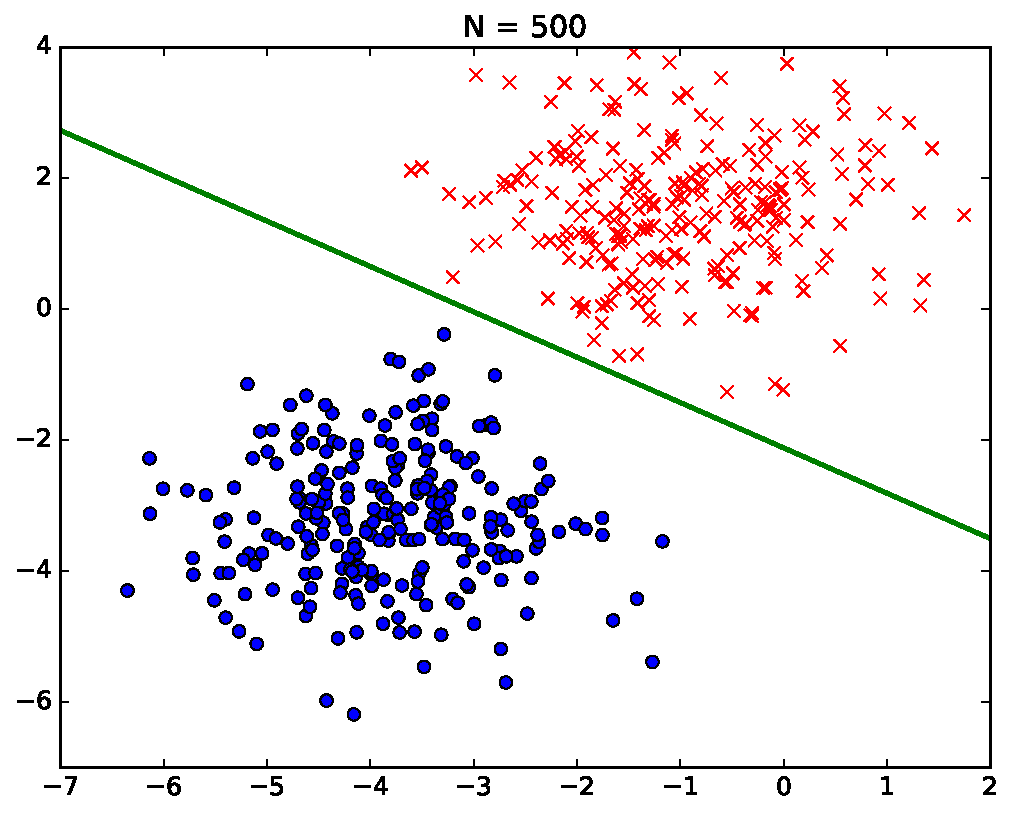
\includegraphics[scale=0.5]{Trial_4/pocket_learning.pdf}
\end{center}
\newpage
\item the linear regression $3$ second to find a hypothesis, and 
\begin{center}
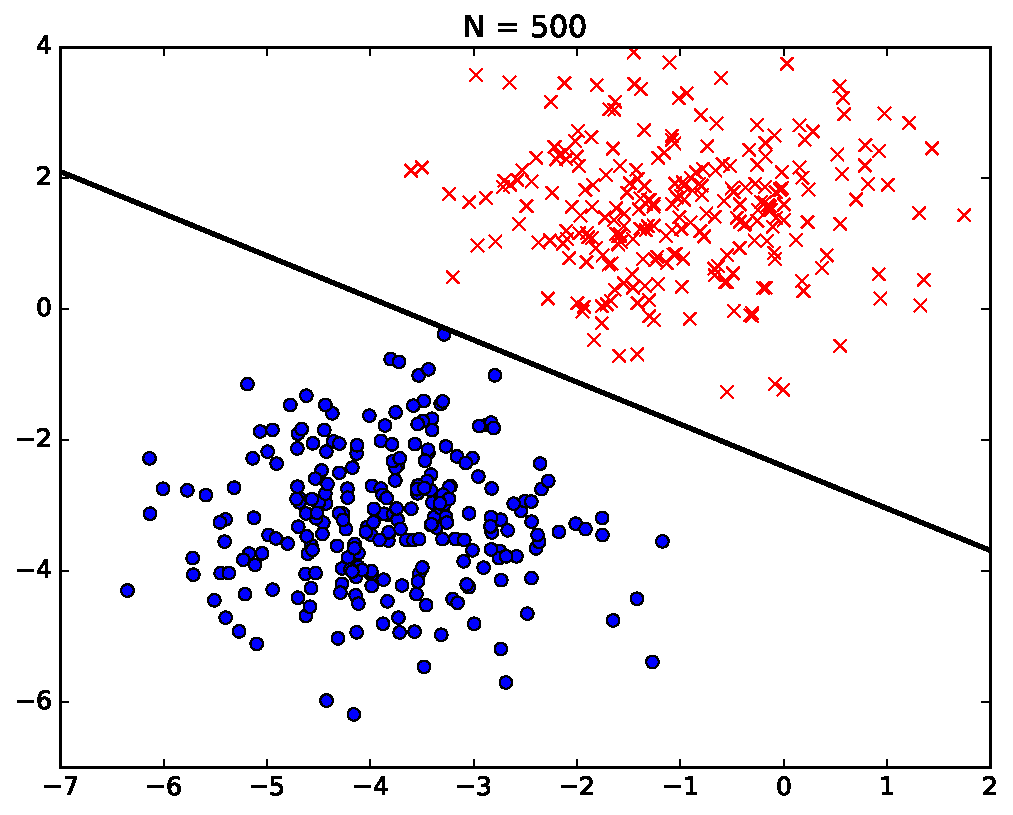
\includegraphics[scale=0.5]{Trial_4/linear_regression.pdf}
\end{center}
\item  the Pocket algorithm using the linear regression solution, $0$ iterations and $3$ seconds to converge.
\begin{center}
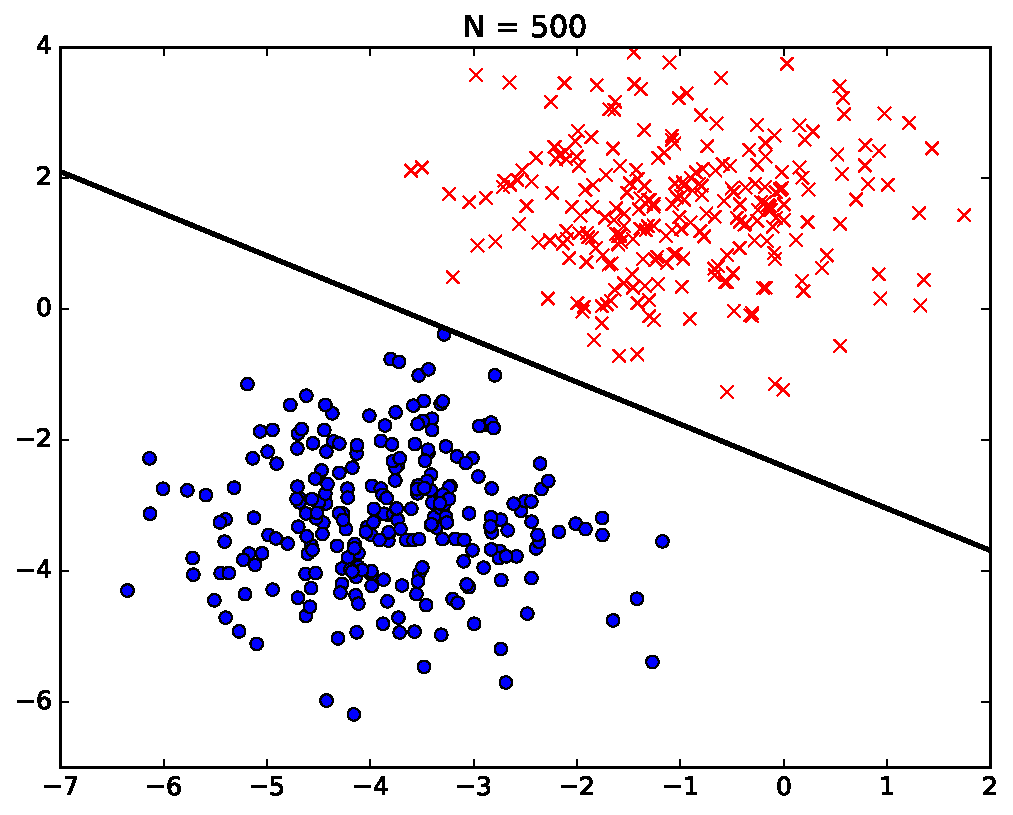
\includegraphics[scale=0.5]{Trial_4/pocket_with_lr.pdf}
\end{center}
\end{enumerate}

The $E_{out} =0$ for all of the approaches, so the the amount of computation required is the most important. The pocket algorithm took the least amount of physical time to find a solution; it was faster by one second. Based on this dataset, it can be concluded that for linearly separable datasets that a pocket algorithm may be advantageous to an approach using linear regression. It should also be noted that the Pocket algorithm using the linear regression solution took zero iterations. This is because the starting weights given by the regression was already produced a classification with no error.

\newpage
Next, a linearly separable data set was examined, both as its original dataset and modified with significant outliers. Without modifications the dataset is obviously linearly separable such that linear regression, used for classification, gives a hypothesis with the least square error and has no misclassification; the Pocket algorithms with a linear regression solution start will give the same hypothesis.

\begin{center}
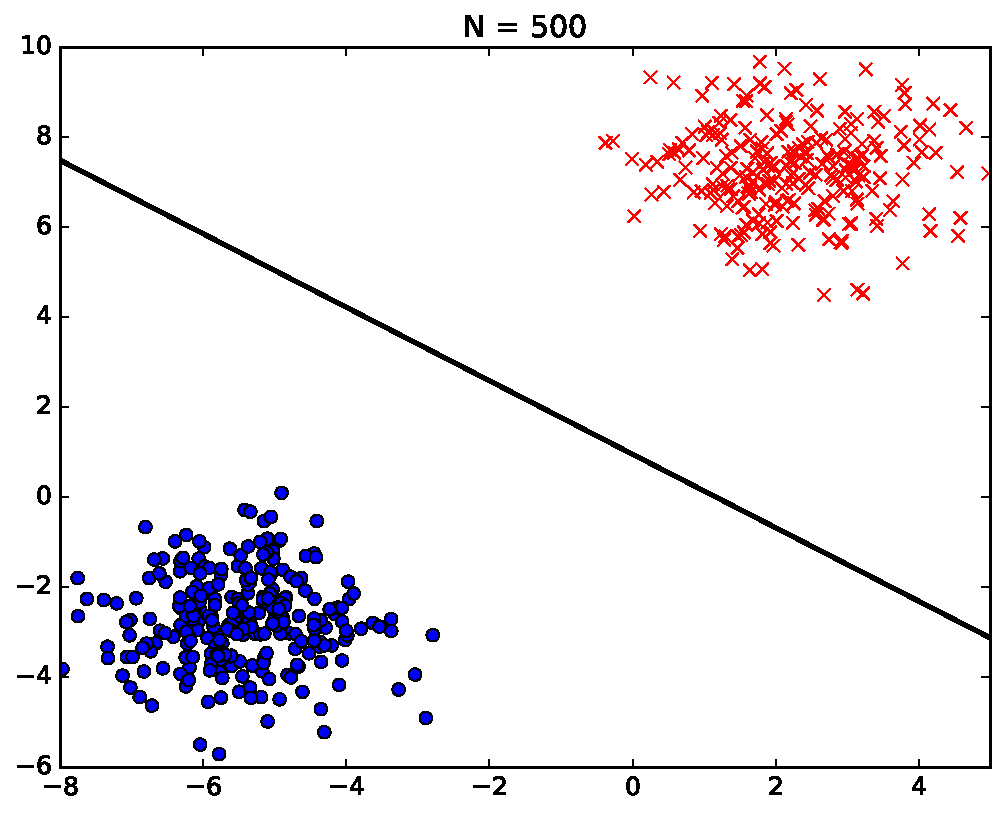
\includegraphics[scale=0.5]{No_Outliers/linear_regression.pdf}
\end{center}

It only took the Pocket algorithm two iterations to produce a hypothesis with no misclassification.
\begin{center}
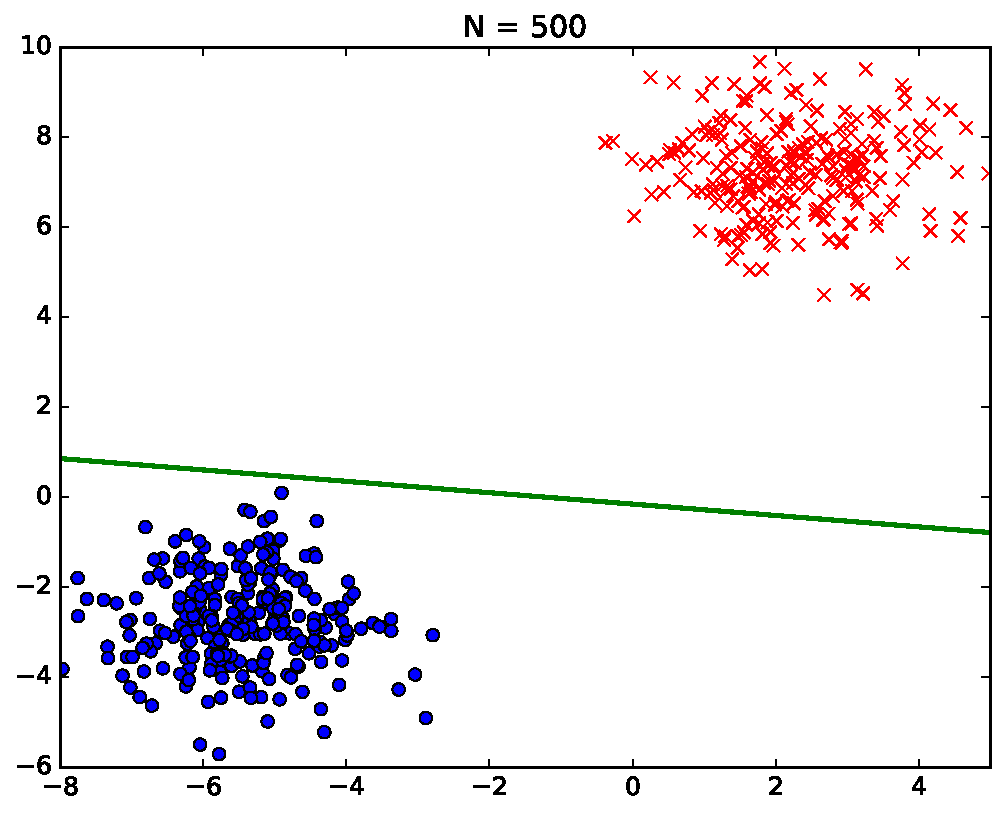
\includegraphics[scale=0.5]{No_Outliers/pocket_learning.pdf}
\end{center}
While there is no misclassification with this hypothesis, the line produced is significantly closer to class 1 than class -1.

\newpage
In order to arbitrarily choose significant outlier to the $y = +1$ class, five of the data points for the $y = -1$ class was modified into the $y = +1$ class. This can be seen in the initial python code shown above, commented out. The only modification that cannot be seen is the the addition to the legend:

\begin{lstlisting}[frame=single]
plt.legend((c0,c1,c2), ('Class -1', 'Class 1', 'Class 1 Outliers'), 
   			loc='upper right',scatterpoints=1, fontsize=11)
\end{lstlisting}

In the plot below, of the dataset with the modification, the purposefully chosen outliers are colored cyan so that they can be easily identified as chosen outliers instead of random outliers.
\begin{center}
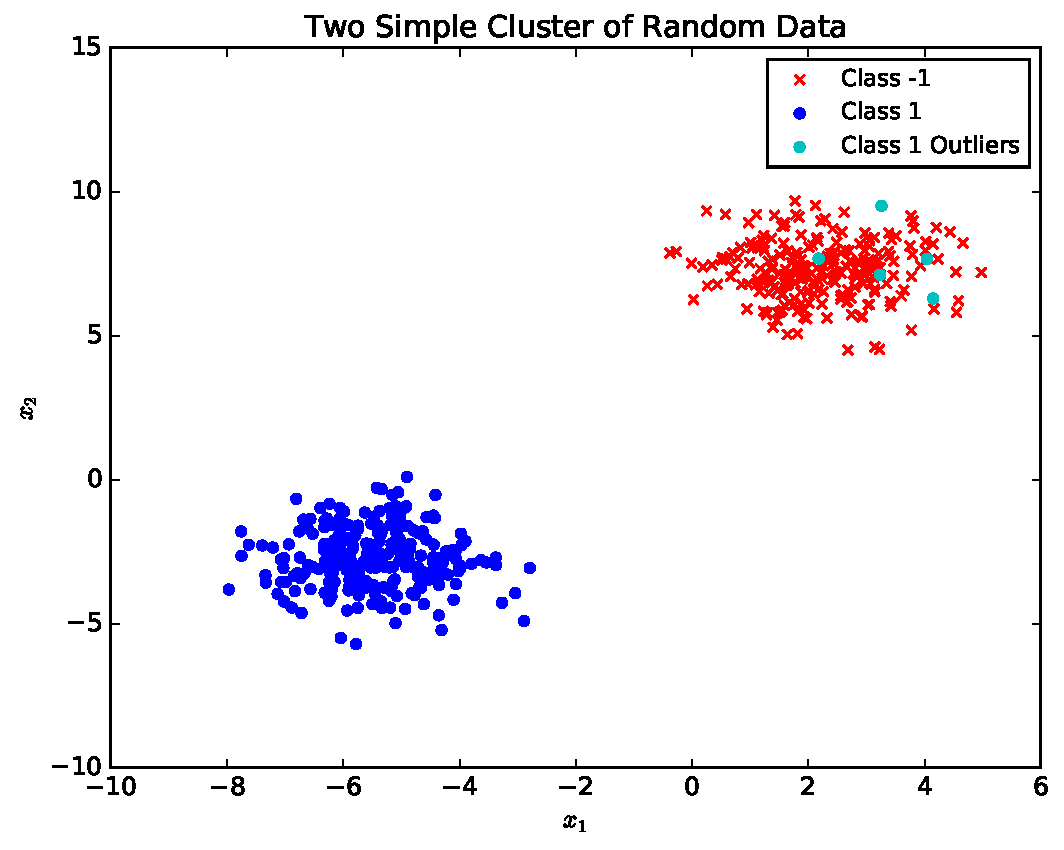
\includegraphics[scale=0.65]{Outliers/hw3_plot.pdf}
\end{center}
With the outliers, the Pocket algorithm and Pocket algorithm with a linear regression start, must wait until convergence at $502$ and $501$ iterations, respectively. It can be seen for all the algorithms, that the final hypothesis does not change from their respective final hypothesis of the dataset without outliers.

\begin{figure}
  \centering
   \caption{Final hypothesis using Pocket algorithm.}
    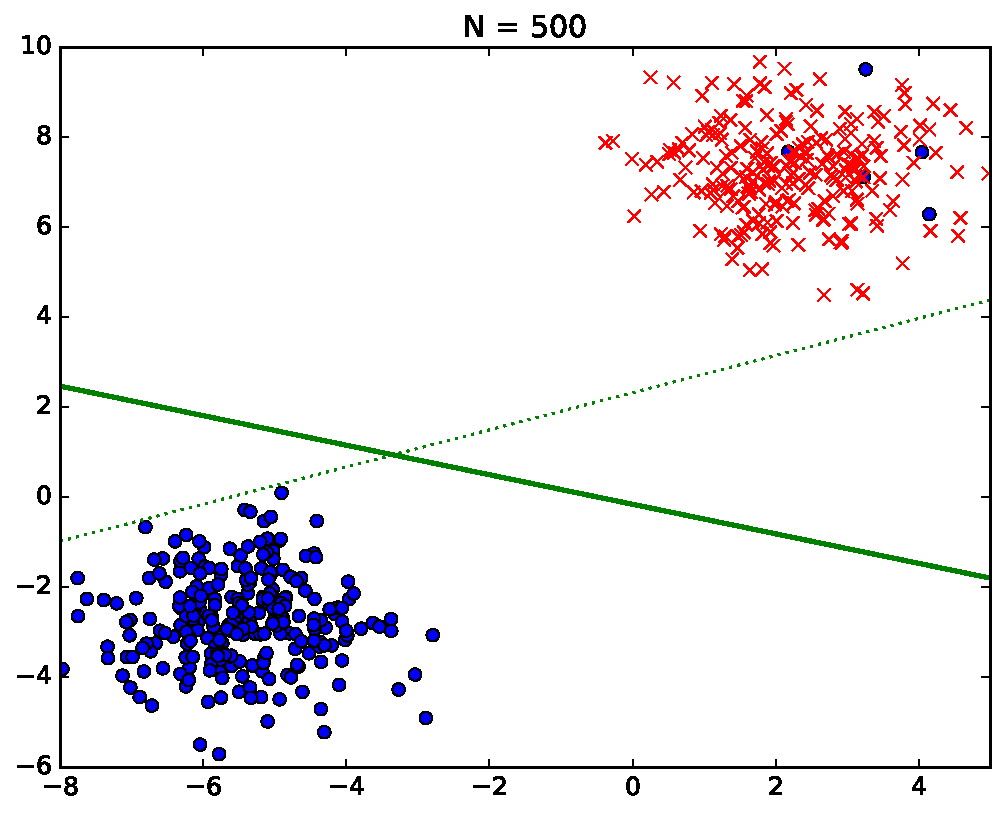
\includegraphics[width=0.45\textwidth]{Outliers/pocket_learning.pdf}
    \bigskip
     \caption{Final hypothesis using linear regression.}
    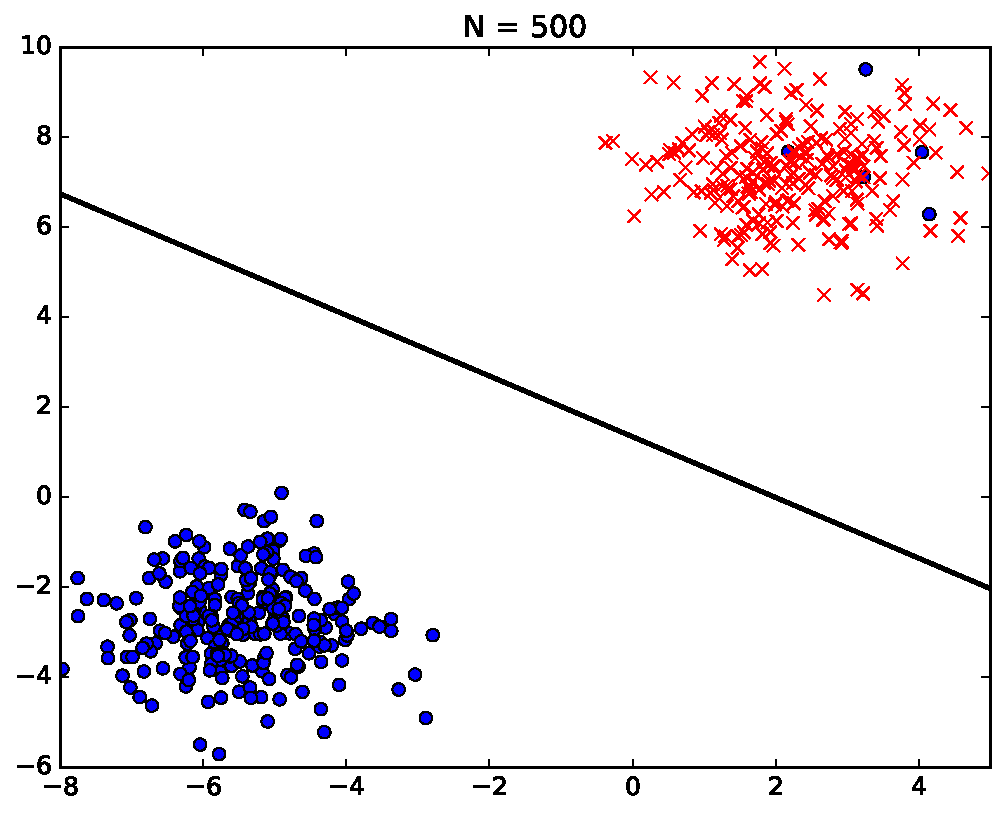
\includegraphics[width=0.45\textwidth]{Outliers/linear_regression.pdf}
    \bigskip
    \caption{Final hypothesis using Pocket algorithm with a linear regression start.}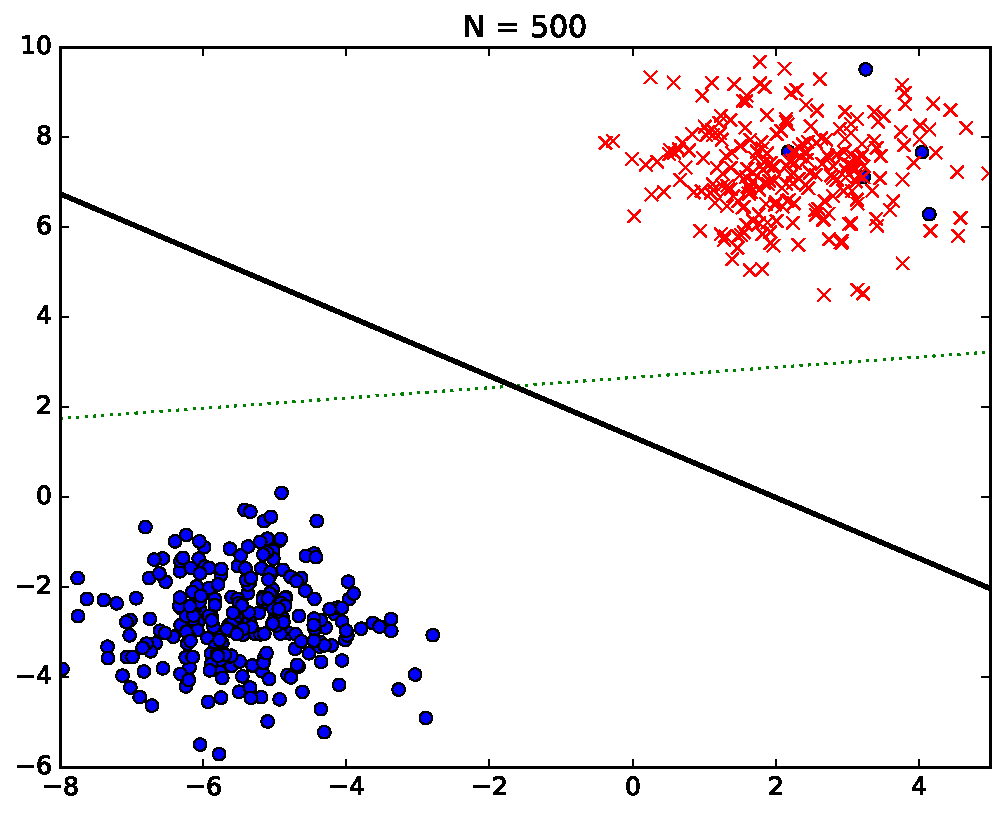
\includegraphics[width=0.45\textwidth]{Outliers/pocket_with_lr.pdf}
     
\end{figure}

In conclusion there are advantages to each of the algorithms, but when the separability of the dataset is unknown it is worth starting the Pocket algorithms with weights from linear regression. It only takes about three second to find the least square error line. The modified Pocket algorithm has all the benefits of linear regression, including ignoring outliers, and the ability to reduce classification error like the perceptron.
\end{doublespace}
\end {description}
\end{document}
